%----------------------------------------------------------------------------------------
%	CHAPTER - INTRODUCTUION
%----------------------------------------------------------------------------------------

\chapter{Introduction} % Main chapter title

\label{ChapterIntroduction} % Change X to a consecutive number; for referencing this chapter elsewhere, use \ref{ChapterX}

%----------------------------------------------------------------------------------------
%	SECTION 1
%----------------------------------------------------------------------------------------

\section{Introduction}

With the public release of the Oculus Rift in March 2016 \citep{Oculus2016} and the HTC Vive in April 2016 \citep{Htcvive2016}, virtual reality has arrived at the consumer level and is all over the news. Although we only see the first iteration of consumer products, \cite{Gartner2015} predicts that within the next five to ten years, virtual reality will achieve mainstream adoption and enter the so called "Plateau of Producitivity". Gesture Control is even a bit ahead of VR and its mainstream adoption is already expected in the next two to five years \citep{Gartner2015}.

The focus of this master thesis is on the possibilities of enhanced user interaction with virtual reality by utilizing not only hand gestures, but making use of the additional sensor information of gesture controllers and 360° motion tracking.

In the following subchapters, more background information about the topic is given as well as the definition of the problem statement. Based on this, the thesis statement is proposed and research questions are derived from. Following this, the delineations and limitations are presented before this chapter is closed with the structure of the thesis and a brief overview of the chapters and their corelations.


%----------------------------------------------------------------------------------------
%	SECTION 2
%----------------------------------------------------------------------------------------

\section{Background}

blub



(Figure \ref{fig:hypecycle}). This means that if Gartner is to be beliefed, Virtual Reality has the phase of over-excitement and unrealistic expectations already behind it and VR is close to the point where it is widely understood by the general public. A bit further than VR itself is Gesture Control that according to \cite{Gartner2015} will already reach mainstream adoption in the next two to five years.
\begin{figure}[h]
	\begin{center}
		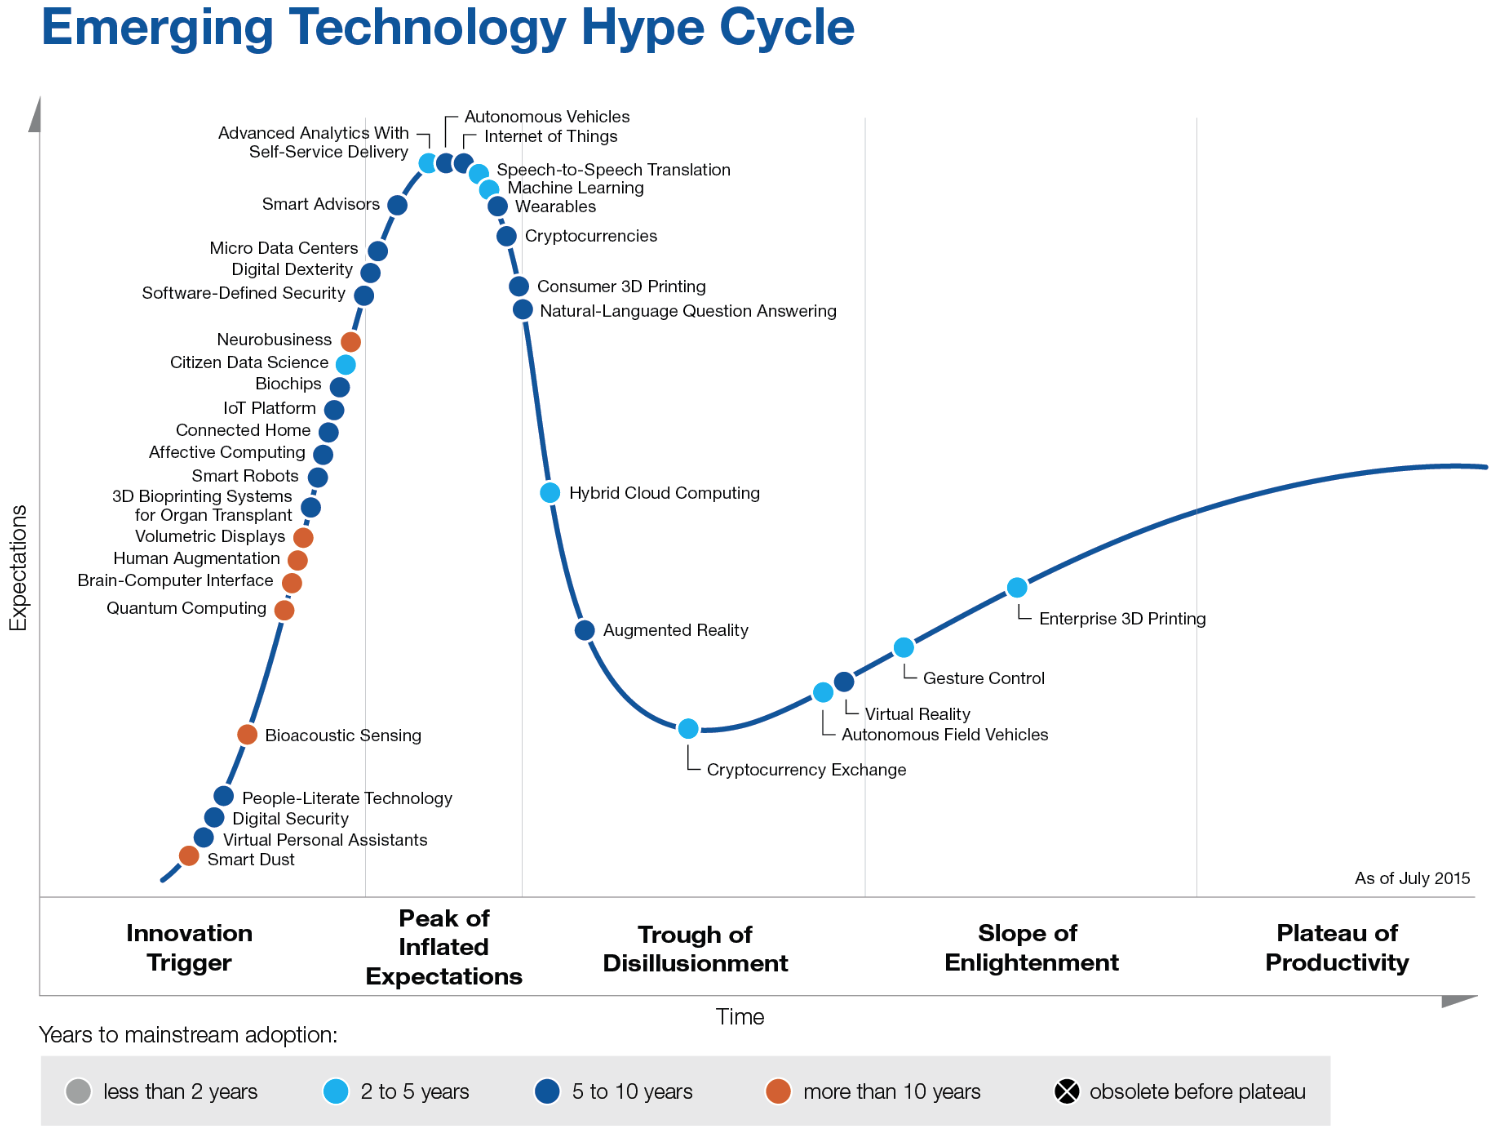
\includegraphics[width=14cm]{03_Figures/03_Gartner/Gartner_EmergingTech2015.png}
		\caption[Emerging Technology Hype Cycle]{Emerging Technology Hype Cycle \citep{Gartner2015b}}
		\label{fig:hypecycle}
	\end{center}
\end{figure}



blub
\cite{Safrudin2015}
blub

%----------------------------------------------------------------------------------------
%	SECTION 3
%----------------------------------------------------------------------------------------

\section{Problem Statement}

blub


%----------------------------------------------------------------------------------------
%	SECTION 4
%----------------------------------------------------------------------------------------

\section{Thesis Statement}

The tesis statement is as follows: \newline
\textit{The interaction with multidimensional data in virtual reality can be enhanced by utilizing gesture controllers and 360° motion tracking.}


%----------------------------------------------------------------------------------------
%	SECTION 5
%----------------------------------------------------------------------------------------

\section{Research question}

To adress the problem statement, research questions are used to break down the research into smaller parts that can be examined individually and allow a view at the nature of the problem from different perspectives.
In this chapter, the main research question (MRQ) as well as the sub research question (SRQ) are formulated. \newline
The main resarch question, derived from the thesis statement, is:
\begin{framed}
	\textit{Can the interaction with multidimensional data in virtual reality be enhanced by utilizing gesture controllers and 360° motion tracking?}
\end{framed} \label{MRQ}
From the MRQ, the SRQs can be derived and are defined as follows:
\begin{framed}
	\textit{SRQ 1: Which ways of interaction with multi-dimensional exist and what are their strengths and weaknesses?}
\end{framed} \label{SRQ1}
\begin{framed}
	\textit{SRQ 2: How can the retrieved sensor information be used to enhance existing interaction patterns with multidimensional data?}
\end{framed} \label{SRQ2}
\begin{framed}
	\textit{SRQ 3: What additional interaction patterns could be possible with the additional sensor data and how can they be integrated?}
\end{framed} \label{SRQ3}
 

%----------------------------------------------------------------------------------------
%	SECTION 6
%----------------------------------------------------------------------------------------

\section{Research Objective}

The research objective of this master thesis is to enhance the interaction with data in virtual reality by proposing the utilization of sensor information from gesture controllers and 360° motion tracking.\newline
This objective will be adressed by first conducting a literature review on the research that has already been done in this field. Based on this a possible prototype will be designed and implemented that will make use if the to be proposed interaction patterns. This also acts as a verification that the interaction patterns indeed are feasible for the currently available technology.


%----------------------------------------------------------------------------------------
%	SECTION 7
%----------------------------------------------------------------------------------------

% \section{Short Overview}


%----------------------------------------------------------------------------------------
%	SECTION 8
%----------------------------------------------------------------------------------------

\section{Delineations and Limitations}

HTC Vive
No speech
focus on

In regards of the design and implementation of the prototype, the artefact will be implemented in Unity3D 5.4 with the SteamVR framework. Although focusing on the technical capabilities of the HTC Vive with its gesture controllers and 360° motion tracking, due to the SteamVR framework functionality (Figure \ref{fig:steamvr}), the reuse of the research for other hardware should be possible in the future. \newline
In addition, with the design and development of a prototype, this thesis focuses more on the technical feasibility than the socioligal aspects of usability, user expercience, or productiviy measurements. 

\begin{figure}[h]
	\begin{center}
		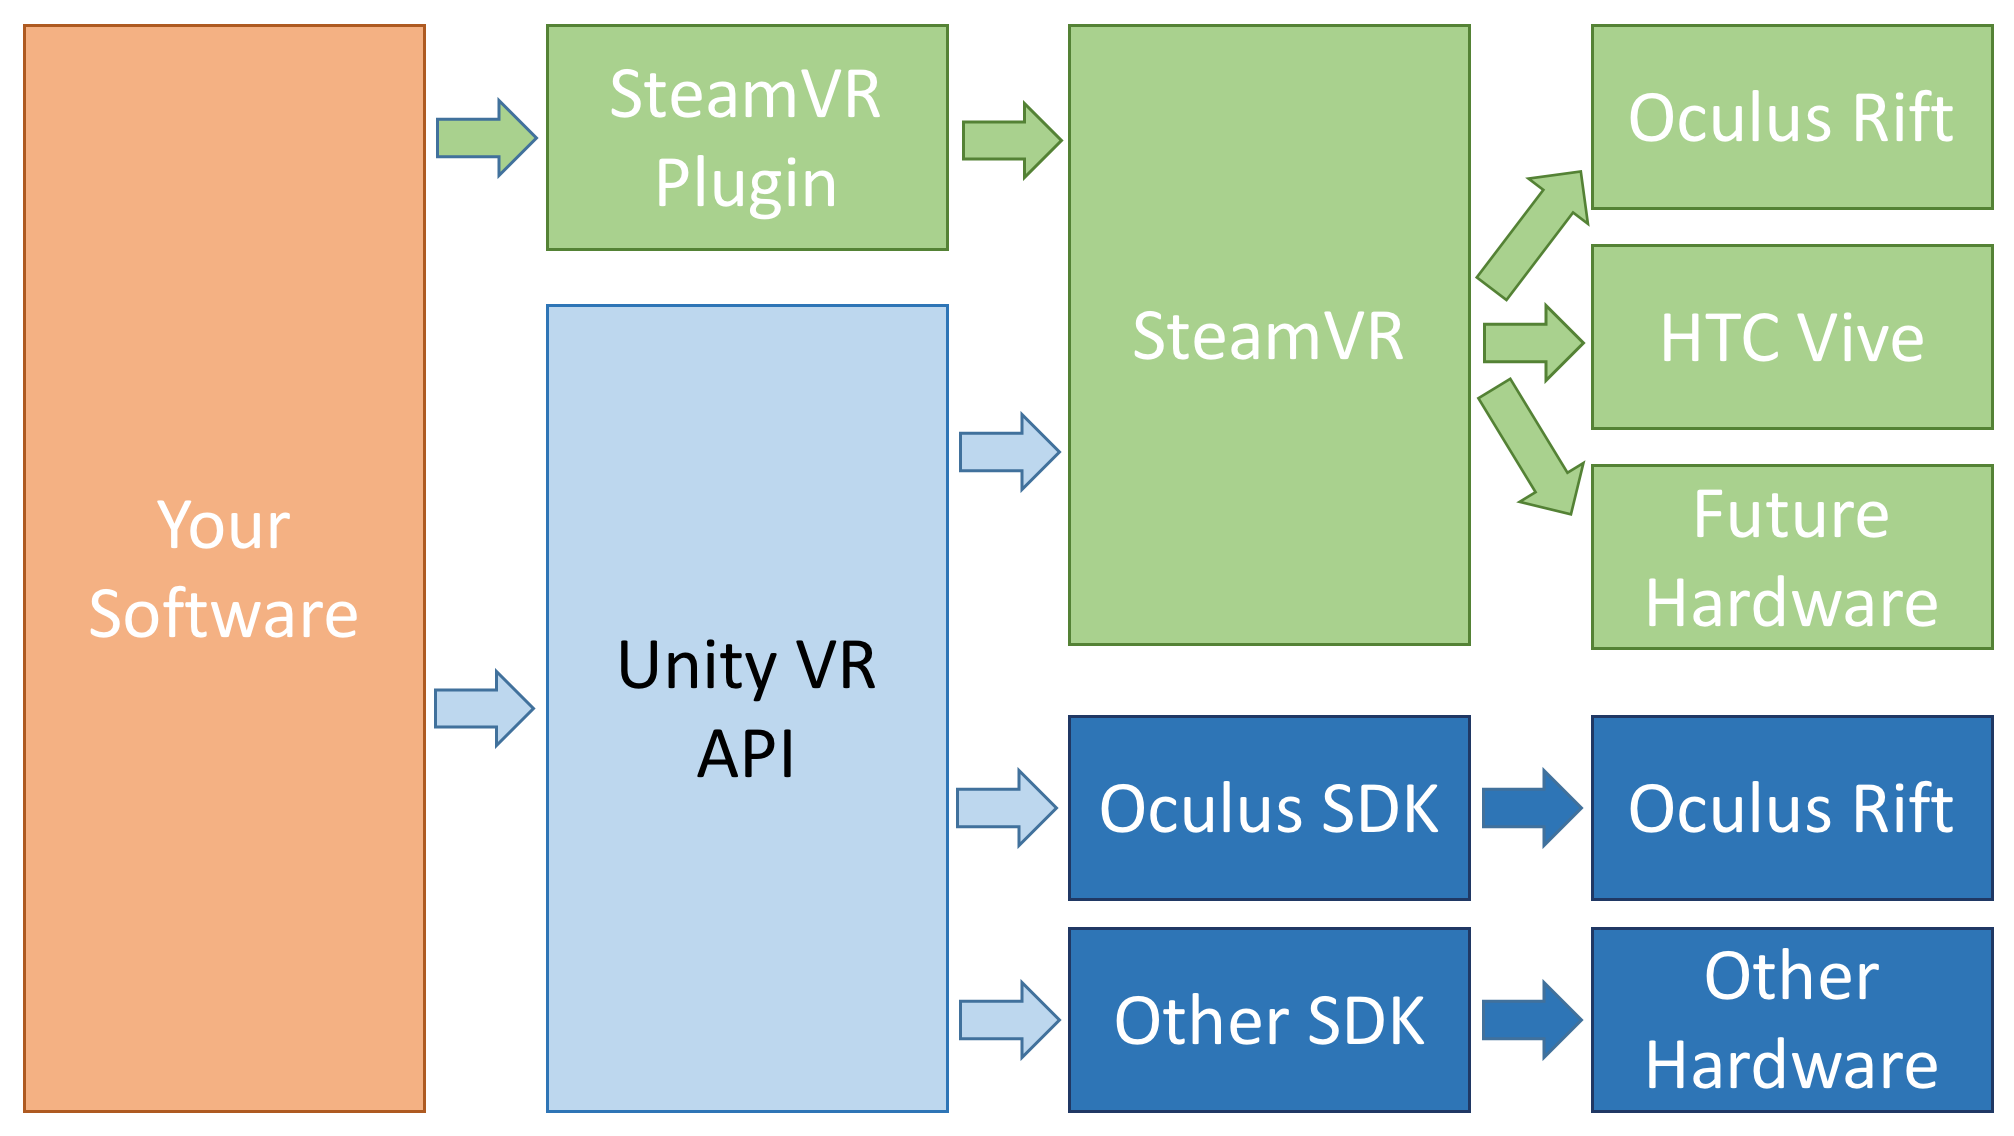
\includegraphics[width=14cm]{03_Figures/04_Valve/OpenVR_SteamVR.png}
		\caption[Steam VR Unity Plugin]{Steam VR Unity Plugin (adopted from \cite{Valve2016})}
		\label{fig:steamvr}
	\end{center}
\end{figure}



Regarding the design and implementation of the Prototype the artefact will be based and optimized on the capability of the Android OS and a chosen smartphone. Nonetheless, the design decision should not restrict the reuse of the research outcome for similar applications and hardware.
With the world getting more and more connected and with the Internet of Things trend (Schwafert, 2015) – smartphones on one part are able to add/retrieve additional information to the tracked sensor data by connecting specific Internet based services (e.g. Points of Interests). In addition, they can also receive actively data from sensors outside the smartphone itself (e.g. sensors of a smart city2). Anyhow, for this thesis, only data that are directly created/received by the built-in sensors are considered – but the scope can be extended for future work.


During the development of the artefact, recommended HCI guidelines provided by the chosen OS manufacturer will be followed (http://developer.android.com/design/index.html) and general consideration to make the app easy to use will be made. However, this thesis focuses more on the technical feasibility – and therefore an in-depth optimization of the HCI and additional usability testing is not foreseen during the development of the artefact.




In this thesis only the Swiss version of the MDS-HC questionnaire is covered. Even though it is similar to the one, which is used in other countries, there are small differences. The questionnaire form is attached to Appendix I.
With regard to sensors, only non-invasive body sensors and environment sensors, which are also called ambient sensors, are used in this study.
1.7 Limitations
Even though invasive sensors are used for different purposes, e.g. blood pressure measurement or blood sugar monitoring (Cleven, Muntjes et al., 2012; Coosemans and Puers, 2005; Tan, Schulam et al., 2013) they are not included in this thesis. For these kinds of sensors it is difficult to find publicly available datasets and so it is not possible to include them in an analysis. Additionally these sensors would require a surgery (Luo, Cheng et al., 2014), which is out of the scope of this master thesis.
Furthermore, data security and privacy are not discussed in this thesis. These are important aspects when information technology is used in the health care domain. Personal health data is very sensitive, however, the focus of this thesis is the mapping of sensors to MDS-HC questions.


%----------------------------------------------------------------------------------------
%	SECTION 9
%----------------------------------------------------------------------------------------

% \section{Underlying Assumptions}


%----------------------------------------------------------------------------------------
%	SECTION 10
%----------------------------------------------------------------------------------------

% \section{Definition of terms and concepts}


%----------------------------------------------------------------------------------------
%	SECTION 11
%----------------------------------------------------------------------------------------

% \section{Significance}


%-----------------------------------
%	SUBSECTION 1
%-----------------------------------

% \subsection{Theoretical}


%-----------------------------------
%	SUBSECTION 2
%-----------------------------------

% \subsection{Practical}


%----------------------------------------------------------------------------------------
%	SECTION 12
%----------------------------------------------------------------------------------------

\section{Thesis structure and brief chapter overviews}

blub


%----------------------------------------------------------------------------------------
%	SECTION 13
%----------------------------------------------------------------------------------------

% \section{Any other institutional requirement not covered here}



